\documentclass[pdf, hyperref={unicode}, aspectratio=169]{beamer}

\usepackage{./diploma-slides-latex-template/styles}
\usepackage{tikz}
\usetikzlibrary{arrows.meta, positioning, fit, backgrounds}

% Включаю кнопочки
\setbeamertemplate{navigation symbols}[default]

% Название темы слишком длинное, поменьше шрифт!
\setbeamerfont{title}{series=\bfseries, size=\large}

\useoutertheme{miniframes}

\graphicspath{ {../pictures/} }

\newcommand{\techlib}[1]{{\scriptsize\itshape\color{black!70}#1}}

\title{Разработка алгоритма лидарной одометрии беспилотного автомобиля, учитывающего перекрытие поля зрения}

\subtitle{Выпускная квалификационная работа студента СпецВО-магистратуры}

\pdfstringdefDisableCommands{
\def\\{}
\def\,{}
\def\textbf#1{<#1>}
}

\author[Инютин Максим Андреевич]
{
	\textbf{Студент группы М8О-206СВ-24:} Инютин Максим Андреевич\\
	\ \textbf{Научный руководитель:} к.т.н., доцент Ухов Пётр Александрович\\
	\ \textbf{Консультант:} Евсеев Дмитрий Сергеевич
	% Обратите внимание на пробел в начале строки
}

\institute[Московский авиационный институт]
{
	Московский авиационный институт (национальный исследовательский университет)\\
	Институт № 8 «Компьютерные науки и прикладная математика»\\
	Кафедра № 806 «Вычислительная математика и программирование» 
}

\date{Москва --- \the\year}

\logo{
\includegraphics[height=1cm]{mai.eps}}


\begin{document}

\epstopdfsetup{outdir=./}

{
	% убирает номер слайда с титульного слайда
	\setbeamertemplate{page number in head/foot}{}
	\frame{\titlepage}
}


\section{Актуальность}
\begin{frame}
	\frametitle{Актуальность: беспилотная отрасль}
	\begin{columns}
		\column{0.40\textwidth}
		\begin{itemize}
			\fontsize{10pt}{12pt}\selectfont
			\item Автономный транспорт уже на дорогах.
			\item Waymo: роботакси в городе.
			\item Яндекс: автономные авто и доставка.
			\item Ключевая задача --- надёжная локализация.
		\end{itemize}
		\column{0.52\textwidth}
		\begin{center}
			\small Waymo\\[0.08em]
			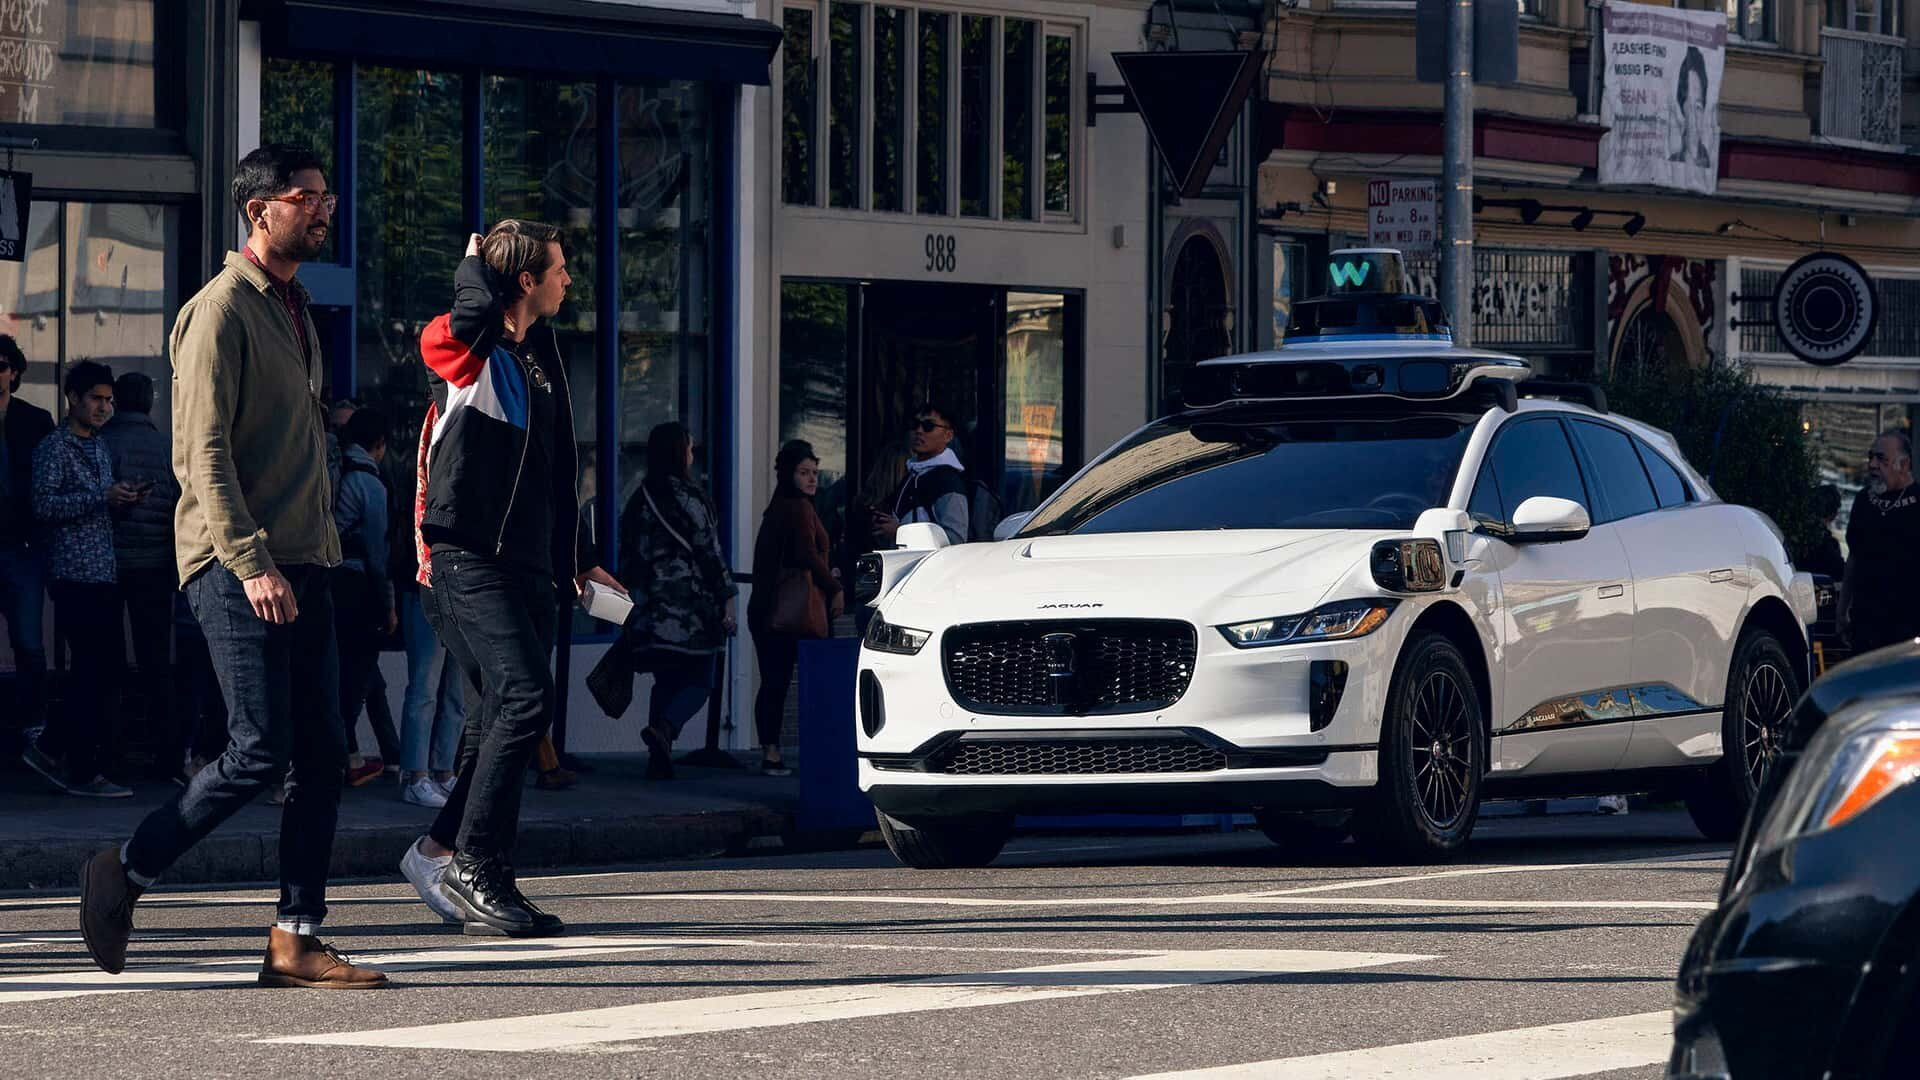
\includegraphics[height=2.55cm, width=0.92\textwidth, keepaspectratio]{waymo-jaguar.jpeg}\\[0.35em]
			\small Яндекс\\[0.08em]
			\includegraphics[height=2.55cm, width=0.92\textwidth, keepaspectratio]{business-robot-pizza.jpg}
		\end{center}
	\end{columns}
\end{frame}


\begin{frame}
	\frametitle{Актуальность}
	\begin{columns}
		\column{0.35\textwidth}
		\begin{itemize}
			\fontsize{10pt}{12pt}\selectfont
			\item GNSS работает нестабильно.
			\item Лидар --- основной источник геометрии.
			\item Грузовик в соседней полосе перекрывает поле зрения и разрушает оценку движения.
		\end{itemize}
		\column{0.55\textwidth}
		\includegraphics[width=\textwidth]{ya/truck-forest.png}\\[0.2em]
		\begin{minipage}{0.49\textwidth}
			\includegraphics[width=\textwidth]{ya/car-field.png}
		\end{minipage}
		\begin{minipage}{0.49\textwidth}
			\includegraphics[width=\textwidth]{ya/car-highway.png}
		\end{minipage}
	\end{columns}
\end{frame}


\section{Цели и задачи}
\begin{frame}
	\frametitle{Объект, предмет, цель и задачи}
	\textbf{Цель:} разработать устойчивый алгоритм лидарной одометрии, сохраняющий оценку движения на коротком участке пути.

	\vspace{0.5em}
	\textbf{Объект:} локализация беспилотного автомобиля по лидарным данным.

	\textbf{Предмет:} алгоритмы лидарной одометрии при перекрытии поля зрения.
	
	\begin{enumerate}
		\item Анализ классических методов регистрации облаков точек;
		\item Формализация сценария перекрытия поля зрения;
		\item Разработка алгоритма: вокселизация, взвешенный ICP, модель движения, фильтр Калмана;
		\item Реализация конвейера и метрик качества;
		\item Экспериментальное исследование на Boreas-RT.
	\end{enumerate}
\end{frame}


\section{Математическая постановка задачи}
\begin{frame}
	\frametitle{Математическая постановка задачи}
	\begin{columns}
		\column{0.55\textwidth}
		По паре соседних облаков $(P_{t-1}, P_t)$ оценить относительное преобразование $T_t$ и скорости $(v_x,v_y,v_z,\omega_x,\omega_y,\omega_z)$.

		\textbf{Образ результата:}
		\begin{itemize}
			\fontsize{10pt}{12pt}\selectfont
			\item Устойчивость к перекрытию поля зрения.
			\item Корректная оценка на 10 секундах ($\sim$ 100 кадров).
			\item Подавление выбросов и учёт кинематики.
		\end{itemize}

		\column{0.45\textwidth}
		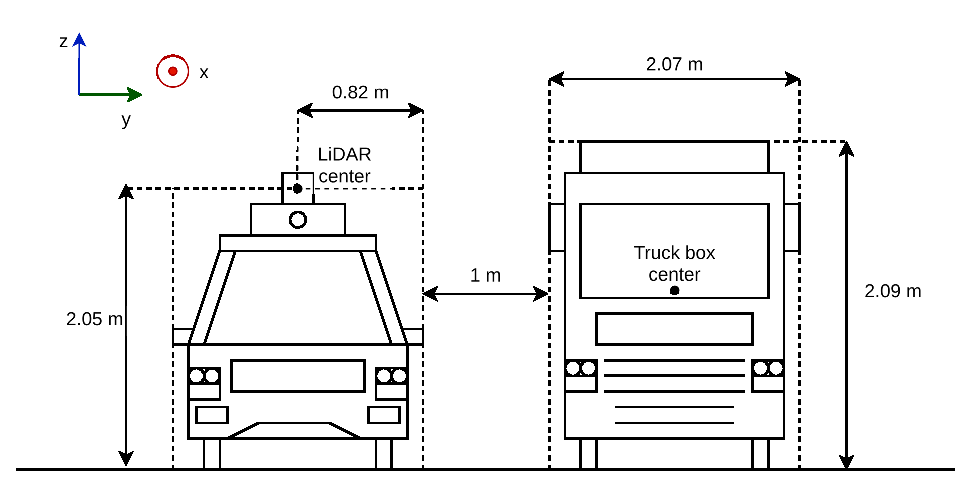
\includegraphics[width=\textwidth]{truck-car-lidar.eps}
	\end{columns}
\end{frame}


\section{Схема решения}
\begin{frame}
	\frametitle{Схема решения}

	\begin{center}
		\begin{tikzpicture}[
			node distance=0.35cm,
			block/.style={rectangle, draw, rounded corners, align=center,
				minimum height=0.9cm, minimum width=2.6cm, fill=blue!10, font=\small},
			arr/.style={-latex, thick}
		]
			\node[block] (pre) {Предобработка\\облака точек};
			\node[block, right=of pre] (vox) {Двойная\\вокселизация};
			\node[block, right=of vox] (init) {Начальное\\приближение};
			\node[block, right=of init] (icp) {Взвешенный\\ICP};
			\node[block, right=of icp] (kal) {Фильтр\\Калмана};

			\draw[arr] (pre) -- (vox);
			\draw[arr] (vox) -- (init);
			\draw[arr] (init) -- (icp);
			\draw[arr] (icp) -- (kal);
			\draw[arr] (kal.south) ..controls +(0,-0.8) and +(0,-0.8).. node[below, font=\footnotesize]{прогноз $\xi_{t-1}$} (init.south);
		\end{tikzpicture}
	\end{center}

	Регистрация --- между двумя соседними облаками.\\Фильтр Калмана стабилизирует начальное приближение ICP.\\[0.4em]
	\small Алгоритм основан на статье \href{https://arxiv.org/abs/2209.15397}{KISS-ICP: In Defense of Point-to-Point ICP}.
\end{frame}


\section{Архитектура решения}
\begin{frame}
	\frametitle{Архитектура решения}

	\begin{center}
		\begin{tikzpicture}[
			node distance=0.32cm,
			block/.style={rectangle, draw, rounded corners, align=center,
				minimum height=1.25cm, minimum width=2.45cm, fill=blue!10, font=\small},
			container/.style={rectangle, draw=black!55, rounded corners,
				inner xsep=0.28cm, inner ysep=0.75cm, fill=gray!6},
			lib/.style={font=\scriptsize\itshape\color{black!70}},
			arr/.style={-latex, thick}
		]
			\node[block] (cfg) {Конфигурация\\эксперимента\\\techlib{JSON, tqdm}};
			\node[block, right=of cfg] (data) {Данные\\Boreas-RT\\\techlib{pyboreas}};
			\node[block, right=of data] (pre) {Облако точек\\и препятствие\\\techlib{NumPy}};
			\node[block, right=of pre] (vox) {Двойная\\вокселизация\\\techlib{NumPy}};
			\node[block, below=0.75cm of cfg] (kal) {Фильтр\\Калмана\\\techlib{NumPy}};
			\node[block, right=of kal] (icp) {Взвешенный\\ICP\\\techlib{cKDTree, align\_vectors}};
			\node[block, right=of icp] (stat) {Метрики и\\статистика\\\techlib{pandas, ttest\_rel, zscore}};
			\node[block, right=of stat] (vis) {Графики и\\ноутбуки\\\techlib{Matplotlib, Plotly, Jupyter}};

			\draw[arr] (cfg) -- (data);
			\draw[arr] (data) -- (pre);
			\draw[arr] (pre) -- (vox);
			\draw[arr] (vox.south) .. controls +(0,-0.65) and +(0,0.65) .. (icp.north);
			\draw[arr] (icp.south) .. controls +(0,-0.65) and +(0,-0.65) .. (kal.south);
			\draw[arr] (kal) -- (icp);
			\draw[arr] (icp) -- (stat);
			\draw[arr] (stat) -- (vis);
			\begin{scope}[on background layer]
				\node[container, fit=(cfg) (data) (pre) (vox) (icp) (kal) (stat) (vis)] (docker) {};
			\end{scope}
			\node[anchor=north west, font=\scriptsize\bfseries\color{black!70}]
				at ([xshift=0.12cm,yshift=-0.12cm]docker.north west)
				{Docker-образ: lidar-odometry-research, основан на python:3.12};
		\end{tikzpicture}
	\end{center}

	\begin{center}\small
		\textbf{Python} --- основной язык реализации; \textbf{Docker} --- воспроизводимая среда.
	\end{center}
\end{frame}


\section{Алгоритмы}
\begin{frame}
	\frametitle{Взвешенный ICP с функцией Гемана---Макклюра}

	Минимизация на каждой итерации:
	\begin{equation*}
		\Delta T = \arg\min_T \sum_{(s,q)} \rho(\|Ts - q\|_2),
		\qquad
		\rho(e) = \frac{e^2/2}{\sigma_t/3 + e^2}.
	\end{equation*}

	\begin{itemize}
		\fontsize{9pt}{11pt}\selectfont
		\item $s \in P_t$, $q \in P_{t-1}$ --- соответствующие точки двух облаков.
		\item $T \in SE(3)$ --- матрица евклидова преобразования $4\times4$, сочетающая поворот и перенос.
	\end{itemize}

	Веса, дающие устойчивость к выбросам:
	\begin{equation*}
		w(e) = \frac{0.5}{\sigma_t/3 + e^2}.
	\end{equation*}

	Решение --- взвешенным алгоритмом Кабша.
\end{frame}


\begin{frame}
	\frametitle{Модель движения и фильтр Калмана}

	\textbf{Постоянная скорость:} прогноз $T_{\mathrm{pred}} = \exp(\xi_{t-1}\Delta t)$.

	\textbf{Фильтр Калмана} по каждой из 6 компонент скорости независимо:
	\begin{center}
		\fontsize{11pt}{13pt}\selectfont
		$Q_v = 0.01$, $R_v = 0.09$, $Q_\omega = 0.01$, $R_\omega = 9\cdot10^{-6}$.
	\end{center}

	\textbf{Оценки шумов:}
	\vspace{-0.4em}
	\begin{columns}[T]
		\column{0.47\textwidth}
		\begin{itemize}
			\item Ускорение автомобиля: 1 м/с$^2$.
			\item Частота лидара: 10 Гц.
		\end{itemize}
		\column{0.47\textwidth}
		\begin{itemize}
			\item Точность лидара: 3 см.
			\item Дальность точки: 100 м.
		\end{itemize}
	\end{columns}

	\vfill
	Главная роль: стабилизация начального приближения ICP на следующем кадре.
\end{frame}


\section{Данные}
\begin{frame}
	\frametitle{Данные: Boreas-RT}
	\begin{itemize}
		\item 10 проездов, 725 десятисекундных сцен; типы: Suburbs, Tunnel, Skyway, Industrial, Farm.
		\item Моделируемый обгон грузовика: смещение $-5$~м, относительная скорость 1~м/с.
	\end{itemize}
	\begin{center}
		\begin{minipage}{0.32\textwidth}
			\centering\small Тоннель\\
			\includegraphics[width=\textwidth]{rides_no_2d/tunnel_truck_overtake_frame_no_2d.png}
		\end{minipage}
		\begin{minipage}{0.32\textwidth}
			\centering\small Трасса\\
			\includegraphics[width=\textwidth]{rides_no_2d/skyway_truck_overtake_frame_no_2d.png}
		\end{minipage}
		\begin{minipage}{0.32\textwidth}
			\centering\small Промзона\\
			\includegraphics[width=\textwidth]{rides_no_2d/industrial_truck_overtake_frame_no_2d.png}
		\end{minipage}
	\end{center}
\end{frame}


\begin{frame}
	\frametitle{Данные: Boreas-RT (продолжение)}
	\begin{center}
		\begin{minipage}{0.45\textwidth}
			\centering\small Сельская местность\\
			\includegraphics[width=\textwidth]{rides/farm_truck_overtake_frame.png}
		\end{minipage}
		\hspace{0.02\textwidth}
		\begin{minipage}{0.45\textwidth}
			\centering\small Пригород\\
			\includegraphics[width=\textwidth]{rides/suburbs_truck_overtake_frame.png}
		\end{minipage}
	\end{center}
\end{frame}


\section{Результаты}
\begin{frame}
	\frametitle{Полные проезды: фильтр не подавляет динамику}
	\begin{columns}
		\column{0.5\textwidth}
		\begin{center}
			\fontsize{8pt}{9pt}\selectfont Без фильтра Калмана\\
			\includegraphics[width=\textwidth]{plots/3_200_500_no_kalman.png}
		\end{center}
		\column{0.5\textwidth}
		\begin{center}
			\fontsize{8pt}{9pt}\selectfont С фильтром Калмана\\
			\includegraphics[width=\textwidth]{plots/3_200_500.png}
		\end{center}
	\end{columns}
	\begin{center}\small Естественные ускорения и замедления сохраняются.\end{center}
\end{frame}


\begin{frame}
	\frametitle{Сцена 341 (Tunnel): устранение деградации $v_x$}
	\begin{columns}
		\column{0.5\textwidth}
		\begin{center}
			\fontsize{8pt}{9pt}\selectfont Без фильтра Калмана\\
			\includegraphics[width=\textwidth]{plots/341_no_kalman.png}
		\end{center}
		\column{0.5\textwidth}
		\begin{center}
			\fontsize{8pt}{9pt}\selectfont С фильтром Калмана\\
			\includegraphics[width=\textwidth]{plots/341.png}
		\end{center}
	\end{columns}
	\begin{center}\small Корректная оценка сохраняется на всех 10 секундах.\end{center}
\end{frame}


\begin{frame}
	\frametitle{Сцена 65 (Tunnel): удержание $v_x$ от провала к нулю}
	\begin{columns}
		\column{0.5\textwidth}
		\begin{center}
			\fontsize{8pt}{9pt}\selectfont Без фильтра Калмана\\
			\includegraphics[width=\textwidth]{plots/65_no_kalman.png}
		\end{center}
		\column{0.5\textwidth}
		\begin{center}
			\fontsize{8pt}{9pt}\selectfont С фильтром Калмана\\
			\includegraphics[width=\textwidth]{plots/65.png}
		\end{center}
	\end{columns}
	\begin{center}\small Фильтр Калмана удерживает $v_x$ около 6 секунд и устраняет смещение $v_z$.\end{center}
\end{frame}


\begin{frame}
	\frametitle{Статистика по 725 сценам}
	\begin{center}
		\fontsize{9pt}{11pt}\selectfont
		\setlength{\tabcolsep}{4pt}
		\begin{tabular}{|l|r|r|r|r|r|r|}
			\hline
			Метрика & mean & std & MSE & MAE & q95 & RMSE \\
			\hline
			\multicolumn{7}{|l|}{\textbf{$v_x$ --- продольная линейная скорость}} \\
			\hline
			A (без фильтра Калмана) & $-0.318$ & $0.299$ & $2.616$ & $0.403$ & $0.835$ & $0.483$ \\
			\hline
			B (с фильтром Калмана)  & $-0.245$ & $0.273$ & $0.775$ & $0.332$ & $0.741$ & $0.409$ \\
			\hline
			Изменение, \% & {\color{green!50!black}$-22.7$} & {\color{green!50!black}$-8.5$} & {\color{green!50!black}$-70.4$} & {\color{green!50!black}$-17.6$} & {\color{green!50!black}$-11.3$} & {\color{green!50!black}$-15.5$} \\
			\hline
			p-value & {\color{green!50!black}$0.033$} & {\color{green!50!black}$0.020$} & {\color{green!50!black}$0.040$} & {\color{green!50!black}$0.030$} & {\color{green!50!black}$0.012$} & {\color{green!50!black}$0.024$} \\
			\hline
			\multicolumn{7}{|l|}{\textbf{$v_y$ --- поперечная линейная скорость}} \\
			\hline
			A (без фильтра Калмана) & $0.068$ & $0.158$ & $0.0490$ & $0.137$ & $0.345$ & $0.180$ \\
			\hline
			B (с фильтром Калмана)  & $0.069$ & $0.154$ & $0.0445$ & $0.135$ & $0.339$ & $0.176$ \\
			\hline
			Изменение, \% & $+1.3$ & {\color{green!50!black}$-2.1$} & {\color{green!50!black}$-9.2$} & {\color{green!50!black}$-1.4$} & {\color{green!50!black}$-1.7$} & {\color{green!50!black}$-1.9$} \\
			\hline
			p-value & $0.94$ & {\color{green!50!black}$<10^{-4}$} & {\color{green!50!black}$0.002$} & {\color{green!50!black}$<10^{-5}$} & {\color{green!50!black}$<10^{-5}$} & {\color{green!50!black}$<10^{-4}$} \\
			\hline
		\end{tabular}
	\end{center}
	\begin{center}\fontsize{9pt}{11pt}\selectfont
		Значимость проверялась парным T-критерием Стьюдента при $\alpha=0.05$.\\
		Основной выигрыш достигается по продольной скорости $v_x$ и поперечной скорости $v_y$.
	\end{center}
\end{frame}


\section{Эффекты и полезность}
\begin{frame}
	\frametitle{Эффекты и полезность}
	\begin{itemize}
		\item Устойчивый алгоритм лидарной одометрии при перекрытии поля зрения.
		\item Снижение MSE по $v_x$ до $-70\%$ на критических сценах.
		\item Сохранение естественной динамики на длинных маршрутах.
		\item Воспроизводимый конвейер для сравнения конфигураций.
		\item Применение: повышение надёжности локализации беспилотного автомобиля при обгоне грузовиком.
	\end{itemize}
\end{frame}


\begin{frame}
	\frametitle{Исходный код и текст диссертации}
	\begin{center}
		
\includegraphics[height=6cm]{qr-git.pdf}
	\end{center}
	\begin{center}\small GitHub: исходный код, конфигурации экспериментов, текст работы.\end{center}
\end{frame}

\end{document}
